\documentclass[UTF8,fontset=fandol,11pt]{ctexart}
\usepackage[a4paper,margin=20mm,headheight=16pt]{geometry}
\usepackage{graphicx,booktabs,tabularx,array,xcolor,enumitem,fancyhdr,hyperref}
\definecolor{purple}{HTML}{7C3AED}
\definecolor{cream}{HTML}{FFF7ED}
\hypersetup{colorlinks=true,linkcolor=purple,urlcolor=purple,pdftitle={MusicaMac 使用说明书}}
\graphicspath{{images/}}
\pagestyle{fancy}\fancyhf{}\fancyhead[L]{\sffamily\color{purple}MUSICA / macOS 使用说明书}\fancyhead[R]{\small v0.3.1}
\fancyfoot[L]{\small 本地播放 · 编号查答案 · 多轮不重复}\fancyfoot[R]{\thepage}
\setlength{\parindent}{0pt}\setlength{\parskip}{6pt}
\setlist{nosep,leftmargin=1.6em,itemsep=4pt}
\renewcommand{\arraystretch}{1.3}
\newcommand{\pathtext}[1]{{\small\texttt{\detokenize{#1}}}}
\newcommand{\note}[1]{\par\smallskip\begingroup\setlength{\fboxsep}{10pt}\colorbox{cream}{\parbox{\dimexpr\linewidth-20pt}{#1}}\endgroup\par\smallskip}
\begin{document}
{\sffamily\Huge\color{purple}MUSICA MAC}\par
{\Large 听歌猜曲 · 安装、升级与使用}\par
v0.3.1\quad /\quad 2026 年 10 月 24 日
\par 主界面左上角与应用图标采用 Musica Logo，资源内置，离线及替换应用后均可显示。
\section*{1\quad 下载、首次安装和覆盖升级}
在 \href{https://github.com/run-luo-tech/MusicaMac/releases/latest}{GitHub Releases} 下载对应架构的 DMG：M 系列芯片选择 arm64，Intel 选择 x86\_64。在苹果菜单“关于本机”可查看芯片类型。普通用户不需要 Source code，也不需要 Python、pip 或额外播放器。
\begin{enumerate}
\item 退出旧版 Musica；已有曲库时先备份下面列出的 \texttt{data} 文件夹。
\item 打开 DMG，将 Musica.app 拖到 Applications。首次使用会安装；已有旧版时选择“替换”。原来放在其他位置的用户，可替换那个位置的同名应用。
\item 从“应用程序”启动新版。ZIP 下载方式也可使用：完整解压，复制其中的 Musica.app 到原安装位置。
\end{enumerate}
\note{\textbf{新装和升级使用同一个包。}歌曲、永久编号、活动记录和个人设置保存在应用外，替换 Musica.app 不会覆盖这些数据。v0.2.0 的 Mac 可用性已由用户确认；v0.3.1 的原生构建与验证结果以对应 Release 为准。}
\subsection*{数据、配置与备份}
\pathtext{~/Library/Application Support/MusicaMac/data}\par
\pathtext{~/Library/Application Support/MusicaMac/config/app.json}
\begin{itemize}
\item Finder 选择“前往 → 前往文件夹”，粘贴上面的路径。
\item 备份前退出软件，复制整个 data，其中包含 library.db 和 audio；不要只复制数据库或只复制歌曲。
\item 升级后可恢复未完成活动。删除应用也不会删除应用外的数据；请自行保管备份。
\end{itemize}
\subsection*{首次打开}
本版本采用临时签名，尚未进行 Developer ID 公证。若 macOS 拦截首次打开，确认下载来源后，在“系统设置 → 隐私与安全性 → 仍要打开”处理该应用。详见 \href{https://support.apple.com/zh-cn/102445}{Apple 官方说明}。
\subsection*{适用环境}
Apple Silicon 与 Intel 分别构建，CI 验收目标为 macOS 14 与 macOS 15；实际构建系统和架构记录在 build-verification.json。活动前请在目标电脑试听声音输出。
\clearpage
\section*{2\quad 导入歌曲和准备主持人答案表}
只导入真实 MP3。推荐文件名：\pathtext{歌手-歌曲名.mp3}，也支持 \pathtext{歌手 - 歌曲名.mp3}；无法提取的字段可在导入预览中补全。
\begin{enumerate}
\item 打开“曲库管理 / 导出答案”，选择文件或文件夹。
\item 检查歌手、歌名和版本备注，确认后导入。软件复制音频并按永久编号管理，原始文件保留。
\item 导出手机 HTML 答案表，传到主持人手机；正式活动前完成准备。
\end{enumerate}
\begin{center}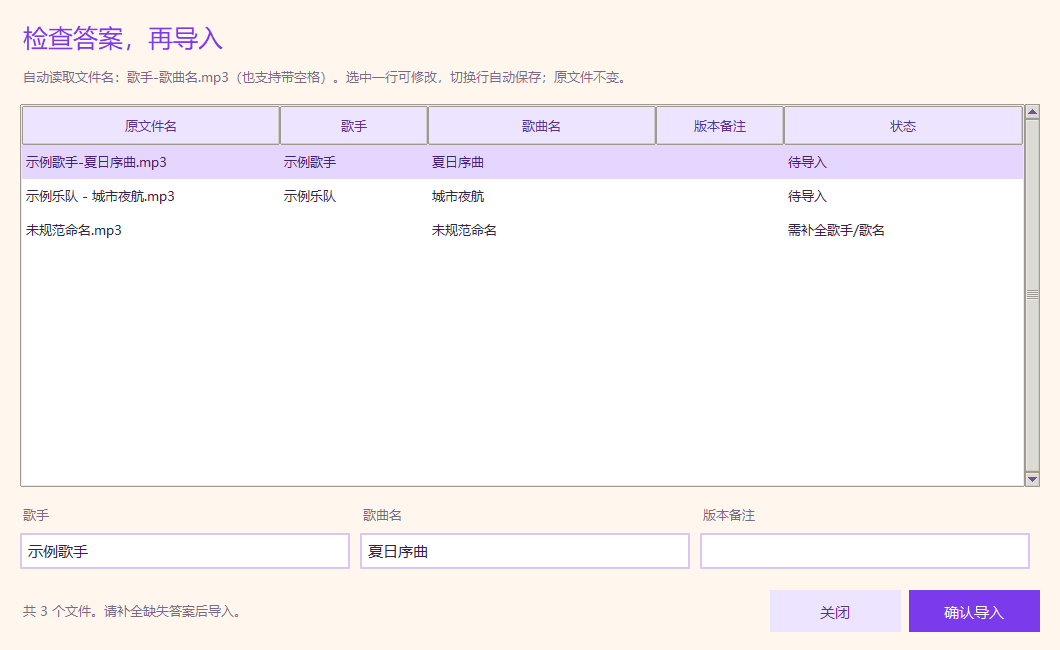
\includegraphics[width=\linewidth]{04-import.png}\end{center}
{\small 图示为 Windows v0.3.1 演示界面；Mac 沿用同一布局和操作，使用 PingFang SC 与 Menlo 字体。示例来自隔离静音曲库，不含用户歌曲。}
\note{\textbf{电脑揭晓前只显示编号。}主持人使用手机离线答案表查编号，避免在共享屏幕中打开包含答案的管理窗口。新增歌曲或修改答案后，需要重新导出手机答案表。}
\subsection*{手机查表和迁移}
手机收到 HTML 后先保存，再用浏览器打开，按编号、歌名或歌手搜索。聊天软件预览可能禁用脚本；必要时可直接查看表格或导出 CSV。

迁移其他电脑的曲库时，先退出两端程序，把完整 data 放到上述 Mac 数据位置。编号、歌曲副本、答案及活动记录会一起迁移，不要在程序运行时覆盖。
\clearpage
\section*{3\quad 播放进度、猜题和活动管理}
\begin{center}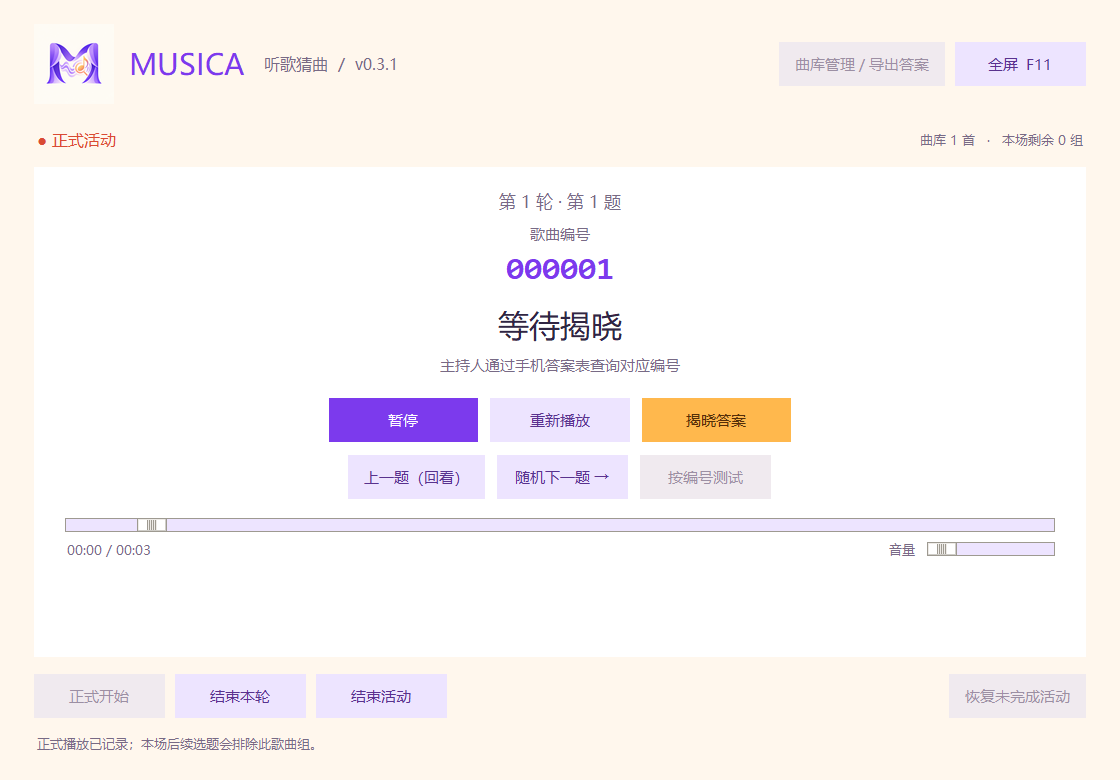
\includegraphics[width=0.72\linewidth]{01-question.png}\end{center}
{\small Windows v0.3.1 演示截图；Mac 操作相同，图中曲目为 3 秒静音夹具。}
\par\noindent\begin{tabularx}{\linewidth}{@{}p{30mm}X@{}}\toprule
操作 & 行为\\\midrule
进度条 & 点击或拖动松开后定位；播放中继续，暂停中保持暂停。\\
预选起点 & 尚未播放时可调整起点，实际播放成功才记录正式题目。\\
键盘定位 & 方向键调整 5 秒，Home 回开头，End 到末尾附近。\\
重新播放 & 始终从开头开始，不重复计题；切题会清除旧起点。\\
揭晓答案 & 作答后展示歌名和歌手；定位不会自动揭晓答案。\\
正式开始 & 创建一场活动，跨轮排除已用歌曲；测试模式不记题。\\
结束本轮 & 保留本场已用记录；可开始下一轮继续活动。\\
退出与恢复 & 未完成活动保留，重开后点击“恢复未完成活动”。\\\bottomrule
\end{tabularx}
\note{MP3 的定位精度取决于编码，不能保证逐采样精确。拖动不会增加正式题数；首次成功播放才计题，即使只播放一小段也视为已用。}
\subsection*{快捷键与验证范围}
F11 切换全屏，Esc 退出全屏，Cmd+Q 退出。正式活动中禁用曲库管理和按编号测试，回看本轮已用题目不重复计数。

新版的自动化验证包括进度控制、记题规则、旧配置和活动保留，以及原生包内 Tk/MP3 播放定位、架构、签名与 DMG 校验。音频夹具为静音，真实扬声器听感仍由主持人在活动前试听。
\end{document}
